\lstdefinelanguage{plaintext}{
  sensitive=false,
  comment=[l]{//},
  morecomment=[s]{/*}{*/},
  identifierstyle=\color{black},
  morestring=[b]',
  morestring=[b]"
}

\lstset
{ 
    language=plaintext,
    basicstyle=\footnotesize,
    numbers=left,
    stepnumber=1,
    showstringspaces=false,
    tabsize=1,
    breaklines=true,
    breakatwhitespace=false,
    frame=leftline
}

\chapter{Implementasi dan Pengujian}
\label{chap:implementasidanpengujian}
Pada bab dijelaskan mengenai implementasi perangkat lunak dan pengujian perangkat lunak. Bagian implementasi berisi tentang lingkungan implementasi dan hasil implementasi.  

\section{Implementasi}
\label{sec:implementasi}
\subsection{Lingkungan Implementasi}
\label{subsec:lingkunganimplementasi}
Implementasi dari perangkat lunak dilakukan pada sebuah laptop. Berikut adalah spesifikasi laptop dan perangkat lunak yang digunakan untuk prapengujian:
\begin{itemize}
\item Processor: Intel Core i3 4030U
\item RAM: 6GB
\item Sistem Operasi: Windows 10 pro 64-bit
\item Versi Apache HTTP Server: 2.4.29
\item Versi MySQL Server: 5.5.5
\item Versi Netbeans: 8.1
\item Versi Google Chrome: 73.0.3683.86
\end{itemize}

\subsection{Hasil Implementasi}
\label{subsec:lingkunganimplementasi}
Hasil dari implementasi adalah sebuah perangkat berbasis terminal yang dapat membangkitkan animasi \textit{timelapse} pada pengembangan proyek perangkat lunak berbasis \textit{web}. Kode program dari perangkat lunak dapat dilihat pada Lampiran \ref{lamp:A}. Setelah dijalankan, perangkat lunak akan menghasilkan dua \textit{output} yaitu, status pada terminal dan \textit{file} hasil animasi bertipe GIF.
\begin{enumerate}
\item \textbf{Status pada Terminal}\\
Setelah berhasil membangkitkan animasi \textit{timelapse}, perangkat lunak menampilkan status pada terminal seperti yang diperlihatkan pada Listing \ref{lst:status_berhasil}. Baris 5 menunjukkan bahwa animasi \textit{timelapse} berhasil dibangkitkan. Pesan pada baris 1-4 muncul saat ChromeDriver membuka dan mulai mengontrol Chrome \textit{browser}.

\begin{lstlisting}[caption={Status pesan pada terminal saat program berhasil membangkitkan animasi \textit{timelapse}.},label={lst:status_berhasil},language=plaintext]
Starting ChromeDriver 2.42.591088 (7b2b2dca23cca0862f674758c9a3933e685c27d5) on port 16446
Only local connections are allowed.
Feb 24, 2019 3:26:25 PM org.openqa.selenium.remote.ProtocolHandshake createSession
INFO: Detected dialect: OSS
Animasi timelapse berhasil dibuat
\end{lstlisting}

\item \textbf{\textit{File} GIF Hasil Animasi}\\
Isi dari \textit{file} GIF hasil animasi dapat dilihat pada Gambar \ref{fig:gif1} - Gambar \ref{fig:gif4}. Gambar \ref{fig:gif1} menunjukkan isi dari \textit{file} GIF jika terdapat satu halaman \textit{web}. Gambar \ref{fig:gif2} menunjukkan isi dari \textit{file} GIF jika terdapat dua halaman \textit{web}. Gambar \ref{fig:gif3} menunjukkan isi dari \textit{file} GIF jika terdapat tiga halaman \textit{web}. Gambar \ref{fig:gif4} menunjukkan isi dari \textit{file} GIF jika terdapat empat halaman \textit{web}. 

\begin{figure}[H]
	\centering
		
\includegraphics[scale=0.4]{Gambar/output1.png}
	\caption{Isi dari \textit{file} GIF jika terdapat satu halaman \textit{web}.}
	\label{fig:gif1}
\end{figure}

\begin{figure}[H]
	\centering
		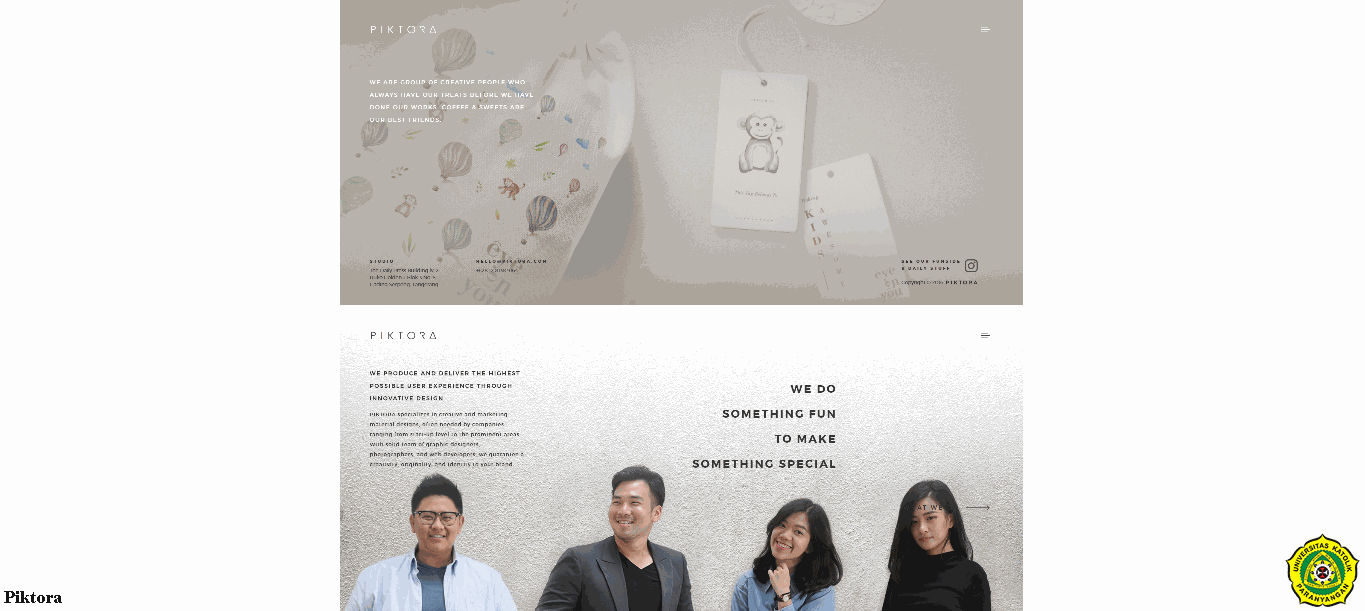
\includegraphics[scale=0.4]{Gambar/output2.png}
	\caption{Isi dari \textit{file} GIF jika terdapat dua halaman \textit{web}.}
	\label{fig:gif2}
\end{figure}

\begin{figure}[H]
	\centering
		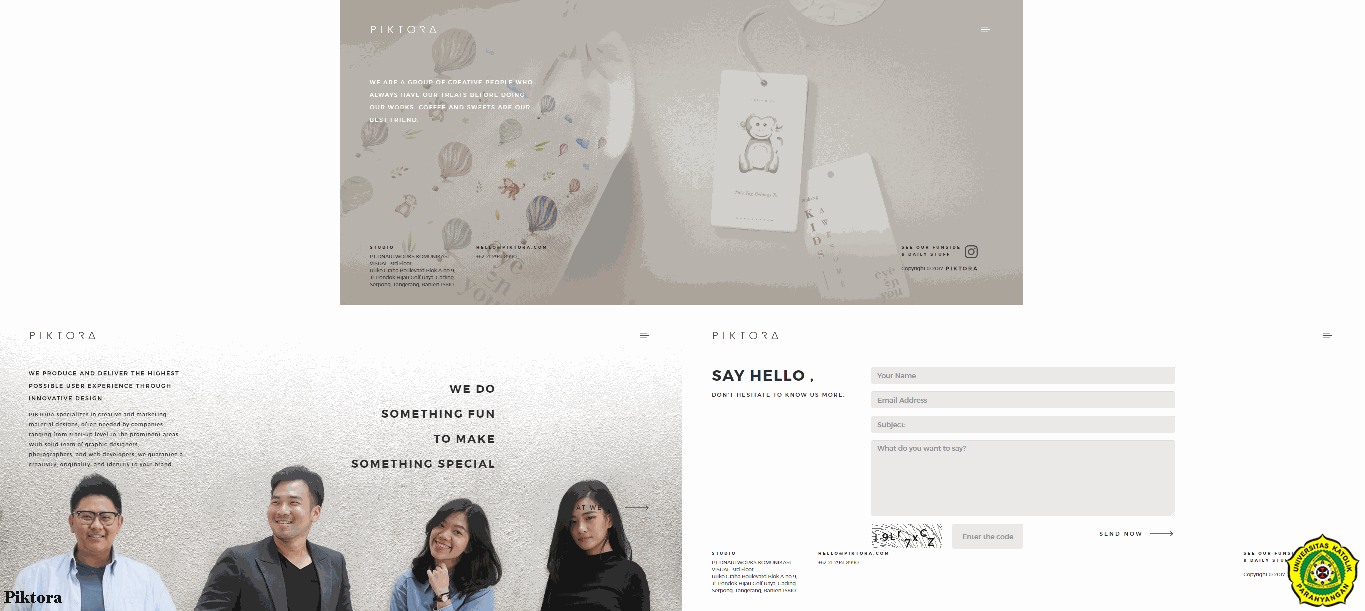
\includegraphics[scale=0.4]{Gambar/output3.png}
	\caption{Isi dari \textit{file} GIF jika terdapat tiga halaman \textit{web}.}
	\label{fig:gif3}
\end{figure}

\begin{figure}[H]
	\centering
		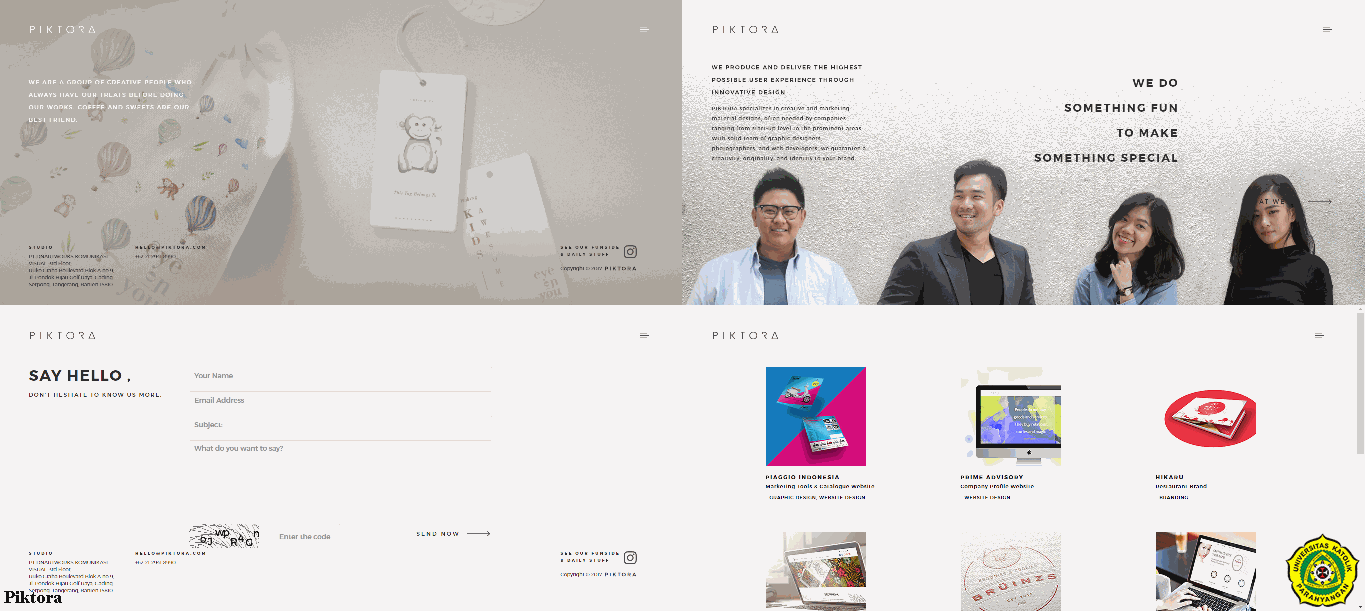
\includegraphics[scale=0.4]{Gambar/output4.png}
	\caption{Isi dari \textit{file} GIF jika terdapat empat halaman \textit{web}.}
	\label{fig:gif4}
\end{figure}

\end{enumerate}
\section{Pengujian}
\label{sec:pengujian}

